\chapter{Ansatz}\label{ansatz}
Nachdem die Problemstellung geklärt ist und die konkurrierenden Technologien erläutert wurden, sollen nun die zugrundeliegenden Gedanken zur Problemlösung vorgestellt werden. Die hier aufgeführten Konzepte für Beispiele verwendete Methoden- oder Klassennamen entsprechen nicht zwingend der tatsächlichen Umsetzung.
\section{Objektstruktur}
Zunächst werden die entsprechenden Modellklassen aus der Xtext Grammatik in Scala Quellcode übernommen. Style-, Shape-, Connection- und Diagram Klassen mit entsprechenden Feldern werden zunächst als sogenannte \textit{case classes} erstellt. Dies hat den Vorteil, dass im Falle einer später notwendigen Verifizierung der Instanzen, vorimplementierte \textit{hash}- \textit{equals}- und \textit{toString} Methoden zur Verfügung zu haben. Da Style am flexibelsten ist (nur eingehende Abhängigkeiten), wird Style.scala zuerst erstellt und entsprechend der Assoziationsreihenfolge dann Shape.scala und Diagram.scala \ref{diagramshapestyle}.
\subsection{ClassHierarchy}Da es für die Instanzen mancher Modellklassen möglich sein soll, Objekte der selben Klasse zu erweitern, ist die Idee des Autors, eine Collection namens \textit{ClassHierarchy} zu erstellen, welche in der Lage ist, ähnlich eines Baumes Vererbungshierarchien in Form von Knoten (\textit{Nodes}) darzustellen. Siehe dazu Abbildung \ref{classhierarchy}. So werden die Modellklassen, für die die Vererbung möglich sein soll, über diesen Baum in Relation gesetzt. Im Falle einer gänzlich neuen Modellklasse (z.B. ein neuer Style), wird die Instanz als neue Basisklasse eingefügt. Ansonsten über eine Methode, die beispielsweise \textit{inheritsFrom} heißen könnte. \textit{InheritsFrom} muss entweder von der \textit{ClassHierarchy} oder den Knoten selber zur Verfügung gestellt werden. Über die entsprechende Argumentenliste wird vermittelt, welche Knoten erweitert werden. \textit{InheritsFrom} ergänzt dann eigenständig die \textit{parent}- und \textit{children} Listen eines Knotens um die neue Instanz der Modellklasse.
\begin{figure}[H]
\begin{center}
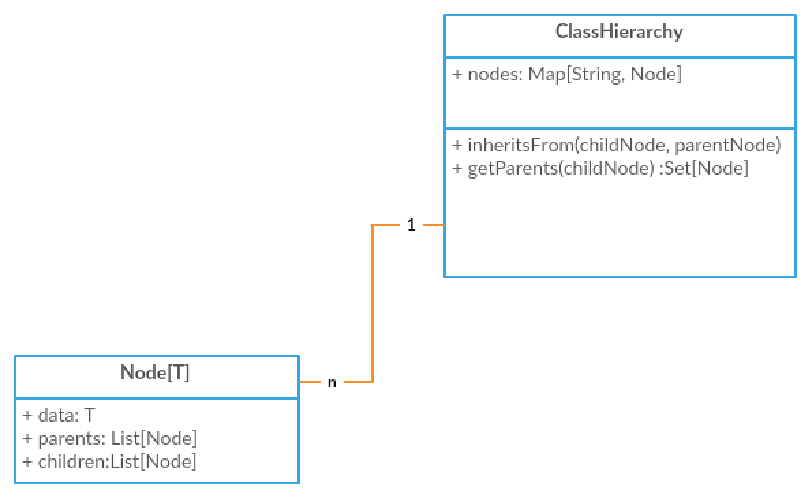
\includegraphics[scale = 0.7]{Bilder/classhierarchy.pdf}
\caption{Klassenmodell von ClassHierarchy}
\label{classhierarchy}
\end{center}
\end{figure}Wie in \ref{classhierarchy} zu sehen ist verfügen die Nodes über Listen, welche auf Eltern- und auf Kind knoten verweisen. So kann man bequem von jedem Style erfahren, welche Styles er erweitert und welche Styles ihn erweitern. Außerdem enthält \textit{ClassHierarchy} eine Map, die Namen (Strings) auf beliebige Klassen abbilden kann. Über dieses mapping ist ein schneller Zugriff auf die gewünschte Klasse möglich, ohne mühsam durch eine Baumstruktur der Nodes navigieren zu müssen.
Um dieses Prinzip auf alle möglichen Klassen anwenden zu können, sollte \textit{ClassHierarchy} generisch sein. Vorausgehend waren die Anforderungen für Vererbung nur auf Style bezogen. Da die Vererbungsprinzipien aber auch bei Shape hilfreich sein könnten, ist so gewährleistet, dass man sich diese Tür nicht unnötig verschließt. 
Benötigte Enumerationen und andere nicht komplexe Hilfsobjekte der Klassen werden in dessen \textit{Companionobject} definiert werden. 
Über entsprechende \textit{Apply}-Methoden wird der Aufruf der \textit{ClassHierarchy} so einfach wie möglich gestaltet (siehe Listing \ref{lst:applyadvance}, Zeile 2).
\begin{lstlisting}[style=scala, caption = {Beispielhafte Vereinfachung durch Apply Methode}, label = {lst:applyadvance}]
classHierarchy.nodes.get("styleName").data
classHierarchy("styleName")
\end{lstlisting}Zeile 1 in Listing \ref{lst:applyadvance} zeigt wie der Aufruf eigentlich ausshen müsste. Zeile 2 hingegen ist kürzer und außerdem verständlicher.
Da der Aufruf in diesem Fall sehr eindeutig ist, kann ruhigen Gewissens auf die Apply-Methode zurückgegriffen werden. "`\textit{Fazit: Die Methoden apply und update sollten nur eingesetzt werden, wenn intuitiv klar ist was der Einsatz der Klammern bedeutet}"'(\Mycite{esser:scala}{76}).

\section{Parser}Neben den Gedanken zur Vererbung der Modellklassen, ist es auch wichtig zu klären, wie die Modelle überhaupt aus der Stringform in Objektform umzuwandeln sind. Entsprechende Mechanismen werden allgemein als Parser bezeichnet. Dieser Parser ist verantwortlich dafür die in Stringform enthaltenen Styles, Shapes, Connections und Diagrams als diese zu identifizieren und in Objekte umzuwandeln. 
Die Struktur eines Styles (ähnlich auch bei den anderen Modellen) ist in Listing \ref{lst:beispielstyle} beispielhaft dargestellt.
\begin{center}
\label{lst:beispielstyle}
\begin{lstlisting}[style=spray, caption={Beispielhafte Style Definition über die entsprechende Style DSL},label={lst:beispielstyle}]
style BpmnDefaultStyle {

	description = "The default style of the petrinet diagram type."
	
	transparency = 0.95

	background-color = black
	
	line-color = black

	line-width = 1

	font-color = black

	font-name = "Tahoma"
	
	font-size = 6

	font-bold = yes

	font-italic = yeshttp://www.macwrench.de/wiki/Kurztipp_-_Quellcodelistings_in_LaTeX

	gradient-orientation = horizontal
	und
}
\end{lstlisting}
\end{center}
Die Xtext Grammatik soll außerdem um eine Vererbungskomponente erweitert werden, die einerseits auch Shapes die Möglichkeit bietet andere Shapes zu erweitern. Zusätzlich soll auch Mehrfachvererbung untersucht und gegebenenfalls umgesetzt werden. Shapes sollen also so definiert werden können wie in Listing \ref{lst:shapeextends} zu sehen ist.
\begin{lstlisting}[style=spray, caption = {(Mehrfach)Vererbung bei einer Shape Definition}, label = {lst:shapeextends}]
shape SomeShape extends StandardShape, AnotherShape {...}
\end{lstlisting}Es ist zwar bereits möglich, Style zu erweitern, doch was die Vererbung von Shapes und Mehrfachvererbung generell angeht besteht noch Bedarf, da Xtext nicht in der Lage ist, diese Features umzusetzen.
\subsection{Parsing Mechanismus und Parserlogik}\label{ansatzlexer}Im Folgenden wird eine konkrete Technik vorgestellt, mit der das Umwandeln, von Strings in Objekte erfolgen kann,
die sogenannten \textit{Regulären Ausdrücke}. Über diese regulären Ausdrücke kann der Style gefiltert werden, um so an der Syntax der DSL vorbei zu kommen und an die eigentlichen Attribute zu gelangen.
Anhand des ersten Wortes, soll der Parser erkennen, um welchen Modelltyp (Style, Shape, Diagram) es sich handelt. 
Weiter würde ein vordefiniertes Schlüsselwort \textit{extends} eine zu erweiternde Instanz kennzeichnen.
Im Gegensatz zu diesen hart kodierten Schlüsselwörtern, werden eigentliche Attribute wie zum Beispiel \textit{line-width} zunächst unter einheitlichen Regeln geparst
und erst in einer tieferen Parser klasse oder dem entsprechenden Konstruktor aufgelöst. Auf diese Art und Weise reichen wenige Regeln aus, um komplexe Ausdrücke abbilden zu können. So geparste Attribute bleiben zunächst in der Stringform. Ziel dieses Vorgehens ist es zunächst nur Attributsname und Attributswert zu ermitteln, sicherzustellen, dass Syntaxregeln eingehalten wurden und die Weitergabe eines einheitlichen Datentyps an tiefer liegende Parserklassen. Diese erste Schicht des Parsers wird also noch keine Objekte, oder gar Baumstrukturen erzeugen, sondern lediglich alle Informationen aus dem String extrahieren, die an einen spezifischen und spezialisierten Parser weiter gegeben werden kann.
Logisch wird hierdurch das Prinzip sogenannter \textit{Lexer} dargestellt, welche insbesondere bei \textit{Compilern} Anwendung finden (vgl. \Myciten{parsing}{135}). Im Prinzip wird ja aber nichts anderes gemacht als eine vordefinierte Sprache zu lesen und umzusetzen, weshalb das Prinzip des Lexers auch hier sinnvoll ist.
Die vordefinierte DSL kann so auch im Bezug auf die Modellklassen leichter modifiziert werden, da solang die Syntaxregeln der DSL nicht geändert werden, der Lexer von neuen Attributen unbeeindruckt ist. Erst die spezifischen Parser müssten bei einer Solchen Änderung um eine Regel erweitert werden, welche in der Lage ist die eigentliche Information aus dem neuen Argument zu extrahieren.
Die wenig komplexen Styles sollten so einfach zu parsen sein. Shapes stellen den schwierigsten Teil beim Parsen dar, da geometrische Figuren(\textit{GeometricModel}), wie Ellipsen oder Polygone ineinander geschachtelt werden können.
\subsection{Factory Klassen}
Es wird davon ausgegangen, dass Modellklassen durch Umwandlung aus einem bereitgestellten Stringinput erzeugt werden. Dieser Stringinput enthält alle notwendigen Informationen um eine einsatzfähige Instanz einer Modellklasse erzeugen zu können. Es ist wünschenswert die Erzeugung der Instanzen so konsistent wie möglich zu halten. Dies bedeutet möglichst wenige und klar definierte Wege ein Objekt zu erzeugen. Dies kann effektiv über eine Fabrik Klasse (zu Englisch \textit{Factory Class}) erreicht werden. Zur Erzeugung der Exemplare der Modellklassen wird so, wenn möglich, nur eine einzige Methode definiert, die schlussendlich auf den Konstruktor der Modellklasse verweist. Dies schließt allerdings noch nicht aus, dass Modellklassen auch anders erzeugt werden können. Scala stellt einen von Haus aus eingebauten Mechanismus zur Verfügung, die \textit{Companion Objekts}. Scala hat sich von den in Java typischen statischen Variablen (Klassenvariablen) getrennt. Um das Prinzip der Objektorientierung konsequenter durchzusetzen, stellt es hierfür die Definition von \textit{Singleton Objekten} zur Verfügung. Über das Schlüsselwort \textit{object} kann anstatt einer Klassen-, eine Objektdefinition erfolgen. Jegliche Felder eines solchen Objekts sind (in Java Manier ausgedrückt) Instanzvariablen, jedoch importierbar. Allein die Möglichkeit auf diese Art und Weise \textit{Singleton Objekte} zu erstellen, deckt bereits eine Funktionalität der Fabrik Klassen ab. Wird ein solches Objekt in der selben Quelldatei wie eine Klassendefinition erstellt und haben Klasse und Objekt außerdem den gleichen Namen, handelt es sich um \textit{Companion Object} und \textit{Companion Class}. Auf den ersten Blick, sind \textit{Companion Objekts} nur der Ansatz Klassenvariablen bereitzustellen und trotzdem dem objektorientierten Paradigma treu zu bleiben. Ein entscheidender Vorteil ist jedoch, dass so definierte Objekte auch auf die privaten Member der \textit{Companion Class} zugriff haben. Auf unseren Fall bezogen bietet sich also die Möglichkeit den Konstruktor der Modellklasse mit dem Schlüsselwort \textit{private} zu kennzeichnen. Folglich kann nur noch das \textit{Companion Objekt} darauf zugreifen und wir können exklusiven Zugriff über eine Fabrik Methode des \textit{Companion Objekts} anbieten. 
\subsection{Parsing Ablauf}
Da in den bisherigen Gedanken geklärt wurde, wie Strings eingelesen werden, die Vererbung unter den Modellklassen dargestellt werden kann und wie Modellklassen konkret erzeugt werden, kann nun anhand des Sequenzdiagramms \ref{sequenzdiagrammAnsatz} beschrieben werden, wie ein Parsing Vorgang prinzipiell abzulaufen hat.\linebreak
\begin{figure}[htb]
	\hspace*{-0.5cm}
		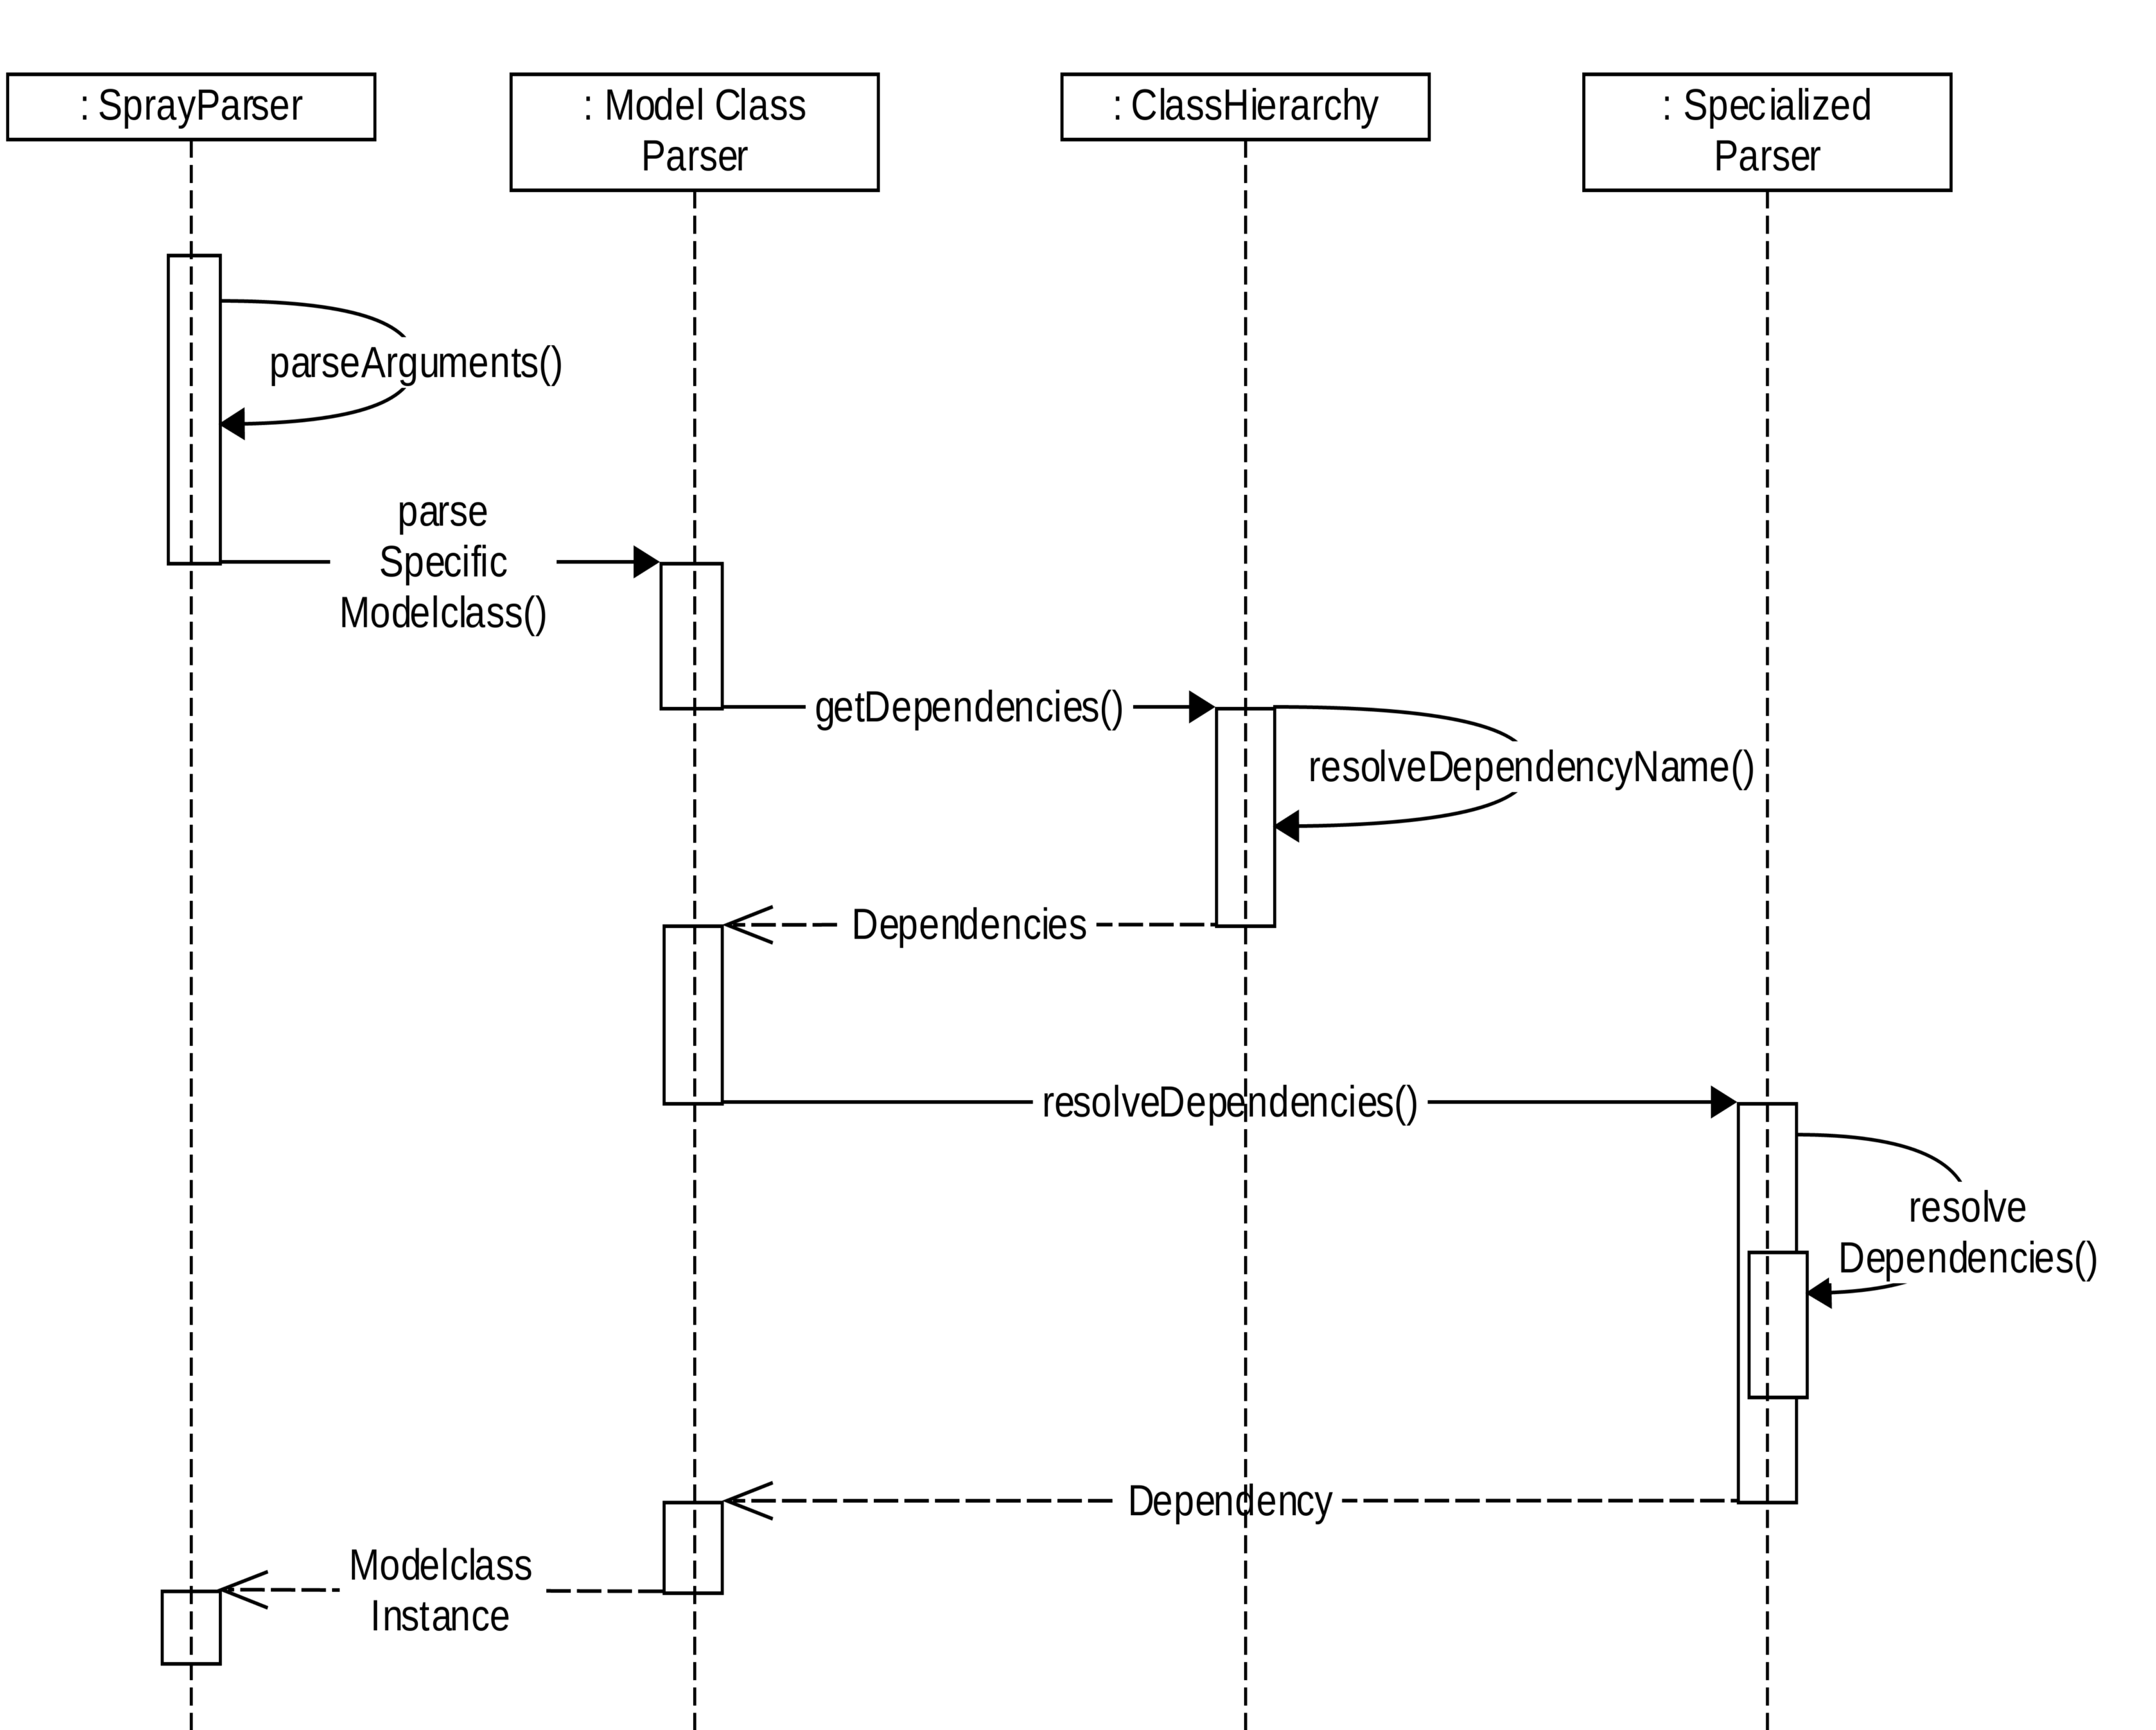
\includegraphics[scale = 0.13]{Bilder/sequenzdiagrammAnsatzKomprimiertScaled(2500x2500).png}
		\caption{Sequenzdiagramm für den Ablauf eines Parsing Vorgangs}
		\label{sequenzdiagrammAnsatz}
\end{figure}Erhält die Applikation einen String um beispielsweise eine Shape einzulesen, werden zunächst sämtliche Attribute aus dem String gefiltert. Hierzu zählen auch Name und erweiterte Shapereferenzen. Dies wird über eine Methode namens \textit{parseArguments}(siehe Abbildung \ref{sequenzdiagrammAnsatz}) erfolgen. Egal um welche Modellklasse es sich handelt, werden alle ausgelesenen Attribute in Stringform weiterverarbeitet. So wird die Verantwortung der Auflösung auf die einzelnen Parser der Modellklassen ausgelagert und diesen gleichzeitig ein einheitliches Medium geliefert. Auf diese Weise können ähnliche oder gleiche Attribute in unterschiedlichen Parsern, auf die selbe Weise aufgelöst werden. Wie bereits angedeutet, geht es von hier an mit einem auf die Modellklasse spezialisierten Parser weiter, der \textit{ModelClassParser}(siehe Abbildung \ref{sequenzdiagrammAnsatz}). Der spezifische Modellklassenparser muss nun zunächst prüfen, ob weitere Instanzen, des Zieltyps erweitert werden sollen. Hierfür gibt er die in den Attributen enthaltene Liste an Eltern (in Form von Strings) an die \textit{ClassHierarchy} weiter, die den Überblick über die Vererbungshierarchie hat und die Namen über ein internes Mapping auf bestehende Referenzen auflösen kann (\textit{resolveDependencyName}, vgl. \ref{sequenzdiagrammAnsatz}). Sind alle Elternteile aufgelöst, kann der modellklassenspezifische Parser nun anhand einer kompletten Liste an Attributen beginnen, die in Stringform enthaltenen Informationen der Abhängigkeiten aufzulösen.
Falls es sich bei den in Stringform enthaltenen Informationen nicht um primitive Datentypen, sondern um komplexe evtl. ineinander geschachtelte Elemente handelt, werden diese wiederum an ihren speziell definierten Parser weitergegeben (\textit{resolveDependencies}, vgl. \ref{sequenzdiagrammAnsatz}). Da die Elemente wie gesagt eventuell ineinander verschachtelt sind, können viele weitere rekursive Aufrufe auf spezialisierte Parsereinheiten erfolgen, bis schließlich alle Argumente aufgelöst sind und eine fertige Instanz an den \textit{SprayParser} zurück geliefert werden kann. Die Parserlogik teilt sich also auf viele kleine spezialisierte Parser auf. Dabei gibt es einerseits den \textit{SprayParser}, der die Schnittstelle zu allen vorhandenen Parsern darstellt, die vier spezialisierten Style-, Shape-, Connection- und Diagramparser, die die Modellklassen erzeugen und einige weitere kleinere Parser, welche dafür verantwortlich sind, eigens erstellte Datentypen parsen und erzeugen zu können, wie zum Beispiel \textit{Anchors}. 
\section{Auflösung von Vererbungshierarchien}
Ist eine Technik gefunden, mit der sich die DSL in die Objektstruktur der Modellklassen umwandeln lässt, muss direkt die Problematik der Vererbung betrachtet werden, da die hierfür benötigten Techniken schon beim Parsen relevant sind. Es soll ein Vererbungsmechanismus implementiert werden. Entgegen der geläufigen Definition der Vererbung, handelt es sich hierbei nicht um das Erweitern von Klassen, so wie man es aus diversen Programmiersprachen kennt. Die Anforderung definiert, dass einzelne Instanzen der Modellklassen in der Lage sein sollen, Objekte der selben Klasse erweitern zu können. Genauer bedeutet dies, dass eine Instanz \textbf{nicht} in der Lage sein soll dynamisch komplett neue Attribute zu definieren, sondern \textbf{bekannte} Attribute von Elterninstanzen zu übernehmen, beziehungsweise zu überschreiben. "`Erweitern"' soll in diesem Kontext also zwei Situationen beschreiben:
\begin{itemize}
\item Elternteil verfügt über Attribute, die in der erweiternden Klasse nicht vorhanden sind -\textgreater Wert wird geerbt
\item Elternteil verfügt über Attribute, die in der erweiternden Klasse vorhanden sind -\textgreater ignoriere/überschreibe den Wert der erweiterten Klasse
\end{itemize}
Das folgende Beispiel soll verdeutlichen, was gemeint ist:
Es wird eine vereinfachte Style Klasse definiert (Listing \ref{lst:beispielstylevereinfacht}).
\begin{lstlisting}[style=scala, caption = {vereinfachte Style Klassendefinition}, label = {lst:beispielstylevereinfacht}]
class Style(val name:String, val transparency:Double, val line-width:Int)
\end{lstlisting}Nun wird eine Instanz \textit{S1} der Modellklasse über die DSL definiert, welche sowohl einen Namen, als auch eine Angabe zur \textit{transparency} hat (Listing \ref{lst:s1}).
\begin{lstlisting}[style=spray, caption = {Style S1}, label = {lst:s1}]
style S1 {
    transparency = 0.5
}
\end{lstlisting}Eine weitere Instanz \textit{S2} wird definiert, die ihrerseits über einen Namen und eine Angabe zur \textit{line-width} verfügt. Außerdem soll \textit{S2} die Instanz \textit{S1} erweitern:
\begin{lstlisting}[style=spray, caption = {Style S2}, label = {lst:s2}]
style S2 extends S1{
    line-width = 10
}
\end{lstlisting}
Nach dem Parsen dieser Definitionen sollten Objekte folgender Struktur entstanden sein (siehe Listing \ref{lst:s1s2json}).
\begin{lstlisting}[style=spray, caption = {\textit{S1} und \textit{S2} Objekte (aus Gründen der Lesbarkeit aufgeführt in der \textit{Java Script Object Notation})}, label = {lst:s1s2json}]
{
 "name": "S1",
 "transparency": 0.5,
 "line-width":"notDefined"
}

{
 "name": "S2",
 "transparency": 0.5,
 "line-width": 10
}
\end{lstlisting}Wie man sieht verfügt \textit{S2} über eine \textit{transparency} Angabe, die von S1 übernommen wurde. \textit{S1} hat von keiner Seite eine Angabe zur \textit{line-width} bekommen. Unternimmt man an dieser Stelle Überlegungen zur Implementierung, wird man mit folgenden Fragen konfrontiert:
\begin{itemize}
\item Wie weiß ein Objekt, dass es das Attribut des Elternteils übernehmen oder überschreiben soll?
\item Übernimmt S2 tatsächlich alle Attribute des Elternteils oder hält es nur eine Referenz auf S1?
\end{itemize}Die meisten der Attribute, die in der Definition einer Modellklasse berücksichtigt werden können, sind optional. Wie man bei der Definition von S1 sieht, wurde keine Angabe zur \textit{line-width} gemacht. Da die Definition jedoch auf den Konstruktor der Style Klasse abgebildet wird, muss irgendwo eine konkrete Angabe zu dem \textit{line-width} Attribut erfolgen. Man könnte sich überlegen, jedem Feld der Modellklassen einen Defaultwert zuzuweisen. Das bedeutet, dass die \textit{line-width} beispielsweise standardmäßig auf 10 gesetzt wird, wenn in der Definition keine Angabe darüber gemacht wird. Hat aber folglich jede Style Instanz zu jedem möglichen Attribut eine valide Angabe, fragt sich, woher später bekannt ist, ob auf Attribute einer Elterninstanz oder auf die eigenen zugegriffen wird. Immerhin gibt es zu jedem Feld der Instanz gültige Werte.
\subsection{Kennzeichnung nicht definierter Felder in Modellklassen}
Da Integer werte ausschließlich gültige Werte haben, ist es sinnlos 0 als \textit{nicht gesetzt} zu verwenden und 1 - \textit{MAX\_INT} als \textit{gesetzte Werte}. Am Beispiel der \textit{line-width} Angabe in S1 wird also klar, dass bekannt sein muss, ob die Definition den Wert beschreibt oder nicht. 
Deshalb werden alle Felder der Modellklassen (Style, Shape, Connection, Diagram), die ein konkretes Attribut der Modellklasse darstellen, als sogenannte \textit{Options} definiert. \textit{Options} sind dem Paradigma der funktionalen Programmierung zu verdanken(z.B. in Haskell -\textgreater Maybe).
Sie lösen ein Problem, welches in Java meist mit einer Exception gelöst wird.
Eine Funktion gibt nicht immer für jedes Argument ein gültiges Ergebnis zurück (vgl. \Myciten{esser:scala}{102}). Im Falle der optional setzbaren Attribute der Modellklassen, bieten Options daher die passende Lösung. Man kann sie entweder auf \textit{None} initialisieren oder auf ein \textit{Some$[$T$]$ }. Repräsentativ steht also in diesem Fall \textit{None} für: "`nicht gesetzter Wert"' (schau in den Elternklassen nach entsprechenden Werten) und \textit{Some$[$T$]$} für: "`gesetzter Wert"', ignoriere/überschreibe den Wert der Elternklasse.
\subsection{Vererbungsmechanismus über Referenz auf Elterninstanzen}
Als nächstes ist es derzeit auch noch unklar an welcher Stelle dieser Gedanke Anwendung findet. Es besteht einerseits die Möglichkeit, erst beim unmittelbaren Zugriff auf die einzelnen Felder zu prüfen, ob sie definiert wurden. Andererseits könnten jegliche Elterninstanzen schon bei der Erzeugung einer neuen Instanz nach fehlenden Werten durchsucht werden. Genauer ist also die Frage, ob Modellklassen eine zusätzliche Referenz auf Elternteile erhalten und nicht definierte Werte erst bei Bedarf in den Attributen der Elternliste gesucht werden oder ob Modellklassen schon bei der Instantiierung über sämtliche Attribute der Eltern Bescheid wissen, diese auf sich übertragen und anschließend nicht mehr auf ihre Eltern angewiesen sind. Beide Möglichkeiten bieten Vor- und Nachteile. Referenzen erlauben es, die Extraktionslogik der Attribute auf eine beliebige Stelle im Code auszulagern, je nach dem wann der Aufruf eben erfolgen soll. 
\subsection{Vererbungsmechanismus durch direkte Weitergabe der Attribute bei Instantiierung}
Werden die Attribute der Elternklasse jedoch direkt bei der Objekterzeugung an die neue Instanz weitergegeben, hat dies zwei besondere Vorteile. Je nach Größe der Vererbungshierarchie ist es wesentlich performanter, die Werte im aktuell benutzten Element zu suchen, als über eine Referenz in den vielen Elternknoten ausfindig zu machen. Außerdem beseitigt diese Vorgehensweise die Rekursivität der Problemstellung. Dazu ein stark vereinfachtes Beispiel:\linebreak Werden mehrere Modellklassen definiert (siehe Listing \ref{lst:allthestyles}), welche den jeweiligen Vorgänger erweitern und wird davon ausgegangen, dass die Attribute der zu erweiternden Instanzen direkt bei der Erzeugung übernommen werden,
\begin{lstlisting}[style=spray, caption = {Definition einiger Styles, die vom jeweils nächsten Style erweitert werden}, label = {lst:allthestyles}]
style S1 {}
style S2 extends S1 {}
style S3 extends S2 {}
style S4 extends S3 {}
\end{lstlisting}kann davon ausgegangen werden, dass \textit{S2} jedes Element von \textit{S1} erbt, \textit{S3} jedes Element von \textit{S2} erbt und somit auch implizit jedes Element von \textit{S1} usw. Der reihe nach werden die einzelnen Styles erzeugt. Wird \textit{S2} erzeugt erbt es direkt alle Attribute von \textit{S1}, die es nicht selbst definiert (und somit gegebenenfalls überschreibt). Wird nun \textit{S3} erzeugt, erbt dieser Style nicht mehr direkt von \textit{S1}, da \textit{S2} garantiert alle Felder von \textit{S1} übernommen oder überschrieben hat. So muss bei der Vererbung also immer nur auf die nächst höhere Elterninstanz zugegriffen werden. Diese Eigenschaft lässt sich auf beliebig viele erweiternde Instanzen anwenden, wodurch in dem Beispiel \textit{S4} garantiert jede Eigenschaft von S1, S2 und S3 enthält, oder überschreibt. Da die Rekursivität der Problemstellung so entfällt und den Code (ausschlaggebender Faktor ist die Größe des durch Vererbung erstellten Baumes) performanter gestaltet, wird versucht die Vererbungshierarchie auf diese Weise aufzulösen.

\section{Generatoren}Ausgehend davon, dass nun Strings eingelesen und in entsprechende Instanzen der Modellklassen umgewandelt werden können, ist der nächste Schritt über Generatoren den nun eigentlich gewünschten Code (Generat) zu erzeugen. Hierfür werden entsprechend der Modellklassen einige Generatorenklassen wie z.B. \textit{StyleGenerator} erstellt, welche die Modellklassen in das gewünschte Format umwandeln. Die Generatorenklassen bilden die entstandenen Objektinstanzen auf \textit{Javascript Code} ab.